\documentclass[a4paper,titlepage]{article}
\usepackage[utf8]{inputenc}
\usepackage{fullpage}
\usepackage{indentfirst}
\usepackage[per-mode=symbol]{siunitx}
\usepackage{listings}
\usepackage{graphicx}
\usepackage{color}
\usepackage{amsmath}
\usepackage{array}
\usepackage[hidelinks]{hyperref}
\usepackage[format=plain,font=it]{caption}
\usepackage{subcaption}
\usepackage{standalone}
\usepackage[nottoc]{tocbibind}
\usepackage[noabbrev,capitalize,nameinlink]{cleveref}
\usepackage{titlesec}
\usepackage{booktabs}
\usepackage{csvsimple}
\usepackage[super]{nth}

% Custom commands
\newcommand\numberthis{\addtocounter{equation}{1}\tag{\theequation}}
\newcommand{\code}[1]{\texttt{#1}}
\newcolumntype{P}[1]{>{\centering\arraybackslash}p{#1}}

\titleformat*{\section}{\normalsize\bfseries}

%opening
\title{
	\textbf{ECSE 526 \\ Assignment 3}
	\\ \large Reinforcement Learning
}
\author{Sean Stappas \\ 260639512}
\date{November \nth{7}, 2017}

\begin{document}
	\sloppy
	\maketitle
	\twocolumn
	
	\section*{Introduction}
	
	
	\section{Description of approach to generalization} \label{sec:generalization_description}
	% 10. provides expression for distance metric between two states and describes state representation used by the RL agent, also includes rationale for choice of components of the distance metric
	
	Q-learning is the learning algorithm chosen for the agent. Many different distance metrics experimented with in the program, as described by Mahadevan and Connell \cite{mahadevan}. Here are three simple distance metrics, with the rationale for each choice of components.
	
	\begin{description}
		\item[Manhattan] The \textsc{Manhattan} distance represents how close two states are on the Qbert pyramid, i.e., the number of blocks between them. This is a natural representation of distance in this environment, since Qbert can only change state by switching blocks and can only travel one block at a time (with the exception of using disks to jump back to the starting position). A distance of 1 was used for \textsc{Manhattan}.
		
		\item[Hamming] The \textsc{Hamming} distance represents the number of different state bits between two given states. The rationale behind this distance metric is that nearby states should have a similar bit pattern, assuming a sane state representation. A distance of 1 was used for \textsc{Hamming}.
		
		\item[SameResult] The \textsc{SameResult} approach groups adjacent states together, such that, whenever a Q-update occurs for a certain Qbert position, all possible states that could have directly led to that state also get updated. The rationale here is that, for most states in the Qbert world, the path Qbert takes to get to that state is usually not important.
	\end{description}
	
	Many different state representations were used with varying results. First, a state representation was used keeping track of the color of every block, the position of disks, Qbert's position, the position of enemies (purple agents) and the position of friendlies (green agents). While this state representation completely encapsulates Qbert's world, it is very verbose and intractable if not using any distance metric, as described previously.
	
	With 21 blocks in the pyramid, an agent has 21 possible positions, representing 5 bits of entropy. This applies for Qbert, the enemies and the friendlies. A simple representation of the colors of the blocks can indicate if the block color is the goal color or not. With this binary value for each block, the colors can be represented with 21 bits. Finally, there are 12 possible locations for the disks, with each disk either being present or not, representing 12 bits of entropy. With all these elements in a state representation, we would need a total of $5*3 + 21 + 12 = 48$ bits to represent a state completely. This represents a state space with $2^{48} \approx 3 \times 10^{14}$ states. Clearly, this number of states is intractable for learning, showing the necessity for generalization with an appropriate distance metric. This state representation is referred to as \textsc{Verbose} in the code.
	
	Another approach to generalization is to use a simpler state representation. A simpler state may not completely represent the game world, but can be enough for an agent to learn how to behave correctly. For example, instead of keeping track of all enemies, blocks and friendlies, one can only keep track of enemies, blocks and friendlies around Qbert, since that is what is important to make an immediate action. One problem with this approach, however, is that it can be hard for the agent to learn to go towards all the blocks in a level to change all the colors and finish the level. More information, such as the number of colored blocks on the board, can then be provided as well. This state representation is called \textsc{Simple} in the code.
	
	Finally, another way to deal with a very large state space is to separate the learning problem into sub-tasks, allowing components of the state to add in complexity instead of multiply. Indeed, if we have separate tasks of enemy avoidance, friendly catching and block finding, we can have a simple specialized state for each task. This is the \textsc{Subsumption} model described by Mahadevan and Connell \cite{mahadevan}, and is explored further in \cref{sec:performance}, where the \textsc{FriendlyCatcher}, \textsc{BlockFinder} and \textsc{EnemyAvoider} learners are described in detail.
	
	To simplify the learning process and avoid recurring sudden death, Qbert's motion is restricted to within the pyramid (with the exception of reaching discs). This allows Qbert to focus on learning to find blocks, avoid enemies and find friendlies.
	
	\section{Results of generalization}
	% 10. results provided for at least 3 different generalization approaches (i.e., choice of components of the distance metric) and meaningful discussion regarding consequences to behaviour of game agent
	
	For all the plots in this report, scores were reported for 100 episodes of playing Qbert. For each episode, Qbert keeps playing until he has no more lives yet, and the total score obtained is recorded. Also, for the following plots showing various generalization results, no exploration is being used.
	
	The results of the Qbert agent with no generalization can be seen in \cref{fig:no_generalization}. We can see that learning takes place relatively slowly because of the massive state space.
	
	\begin{figure}[!htb]
		\centering
		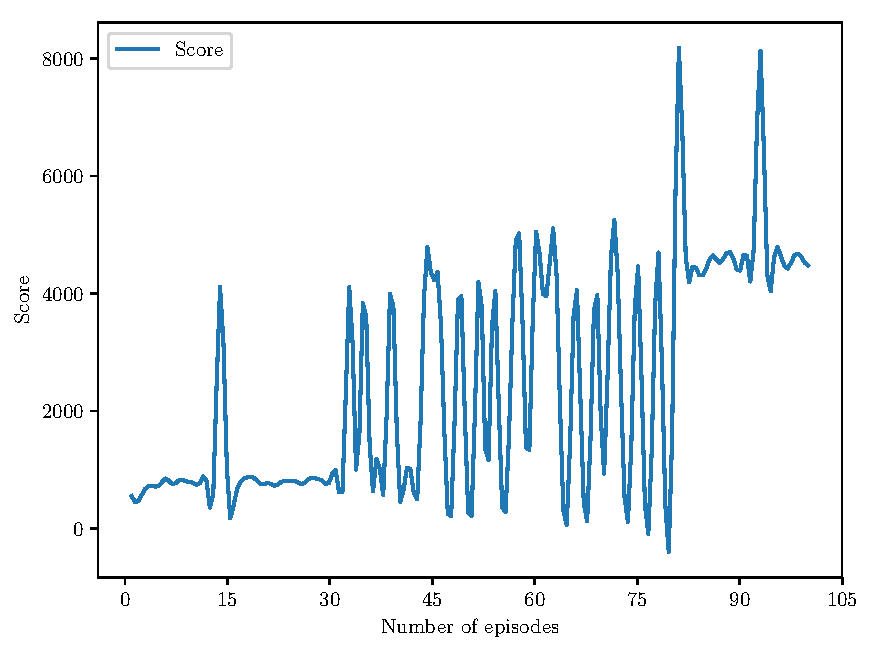
\includegraphics[width=\columnwidth]{plots/no_generalization.pdf}
		\caption
		{Score achieved by the agent with no generalization and no exploration.}
		\label{fig:no_generalization}
	\end{figure}

	The results of the Qbert agent using the \textsc{Manhattan} distance metric can be seen in \cref{fig:manhattan}. It seems that learning is actually hindered with this metric, with overall lower scores being obtained. This may be explained by the fact that assigning the same Q-value to adjacent states may not always be wise. For instance, if Qbert dies to an enemy at a specific block, it probably doesn't make to assign the same penalty to all nearby blocks.

	\begin{figure}[!htb]
		\centering
		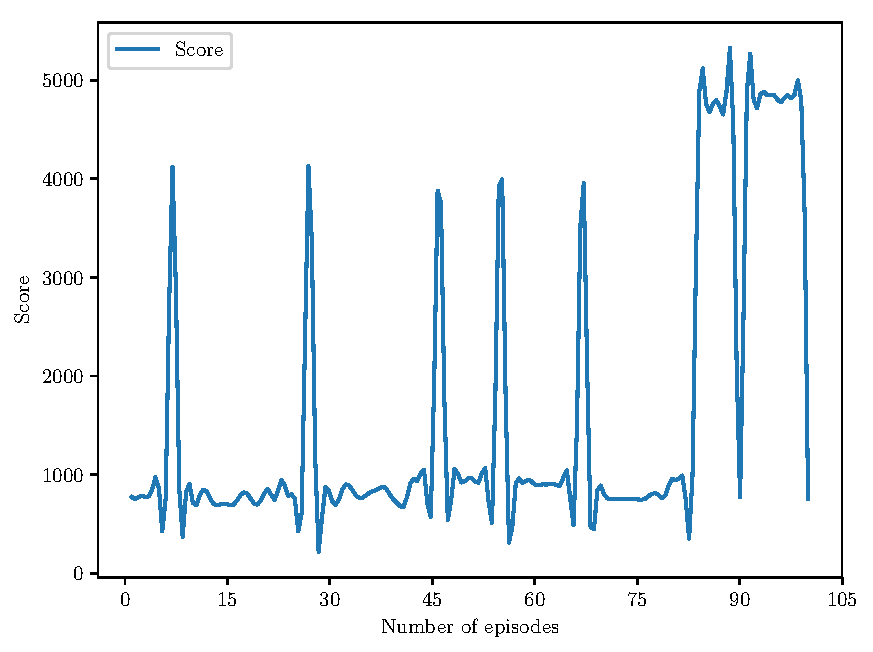
\includegraphics[width=\columnwidth]{plots/manhattan.pdf}
		\caption
		{Score achieved by the agent using the \textsc{Manhattan} distance metric.}
		\label{fig:manhattan}
	\end{figure}

	The results of the Qbert agent using the \textsc{Hamming} distance metric can be seen in \cref{fig:hamming}. While the learning converges relatively quickly to a score, it clearly fails to converge to a very high one. Once again, the distance metric may have caused unintended states to have the same reward, causing repetitive destructive behaviour.

	\begin{figure}[!htb]
		\centering
		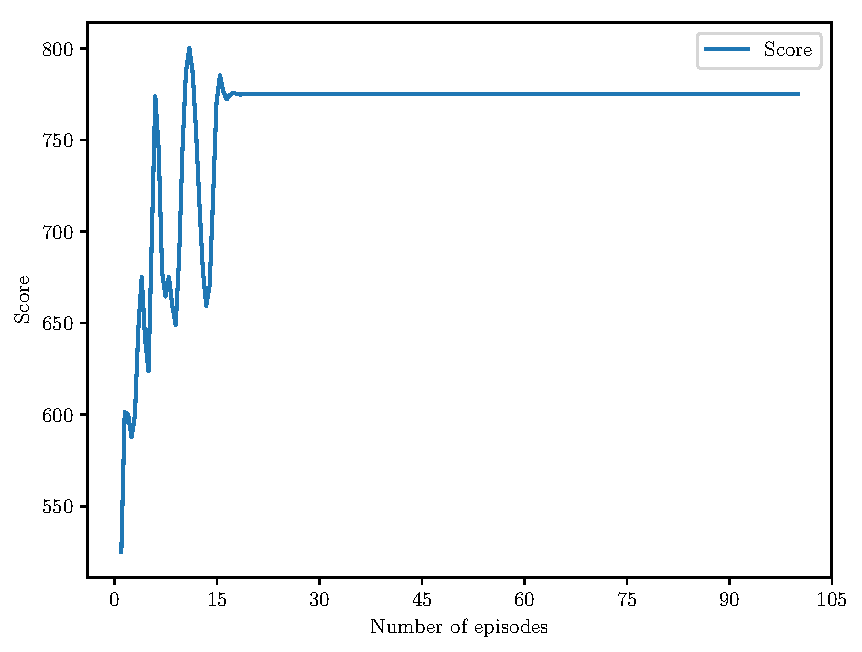
\includegraphics[width=\columnwidth]{plots/hamming.pdf}
		\caption
		{Score achieved by the agent using the \textsc{Hamming} distance metric.}
		\label{fig:hamming}
	\end{figure}

	The results of the Qbert agent using the \textsc{SameResult} distance metric can be seen in \cref{fig:same_result}. Here, the distance metric clearly failed to provide learning, with the score converging to a lower value than the starting one. By assigning the same utility to states that lead to the same other states, the agent has degenerated to repetitive behaviour, leading to easy prey for the purple enemies.

	\begin{figure}[!htb]
		\centering
		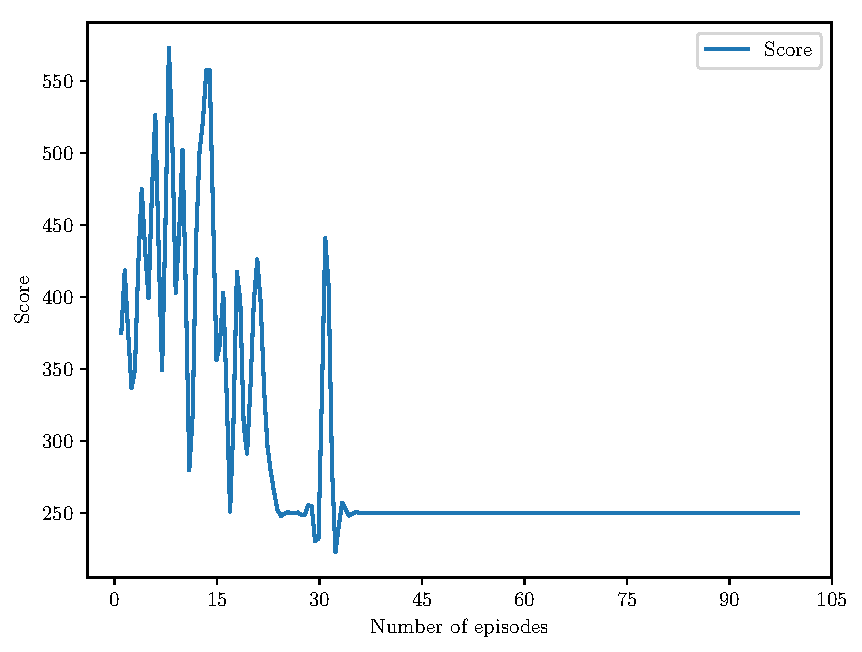
\includegraphics[width=\columnwidth]{plots/same_result.pdf}
		\caption
		{Score achieved by the agent using the \textsc{SameResult} distance metric.}
		\label{fig:same_result}
	\end{figure}

	It is clear that all the described distance metrics have not been successful. This can be explained by the simple fact that, even with distance metrics, the \textsc{Verbose} state space is much too big. To address this issue, we have created a \textsc{Subsumption} agent using the \textsc{Simple} state representation. The details of this model will be described in \cref{sec:performance}, but its performance as a generalization technique can be seen in \cref{fig:subsumption_generalization}. Here, we see a clear upward learning trend despite the spiky data. Note that the spikiness in the data is due to the great danger in the Qbert world, where death is very easy near purple enemies.

	\begin{figure}[!htb]
		\centering
		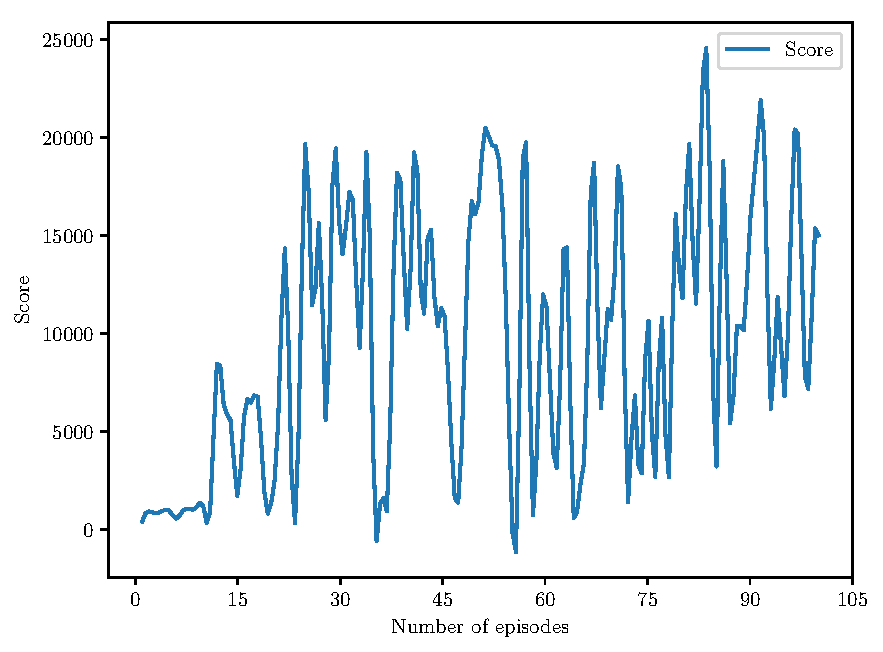
\includegraphics[width=\columnwidth]{plots/subsumption_generalization.pdf}
		\caption
		{Score achieved by the \textsc{Subsumption} agent using a \textsc{Simple} state representation.}
		\label{fig:subsumption_generalization}
	\end{figure}

	Note that exploration has been completely ignored here, since it will be discussed in the next section. This explains the relatively mediocre score results. It should be noted, however, that with the subsumption model, the agent learns with the \textsc{EnemyAvoider} quickly enough to avoid purple enemies, and this acts in a way as a form of exploration, since the enemies will force Qbert to go around the pyramid to avoid death. Indeed, this will force Qbert to visit states that he would normally not visit.
	
	\section{Description of approach to exploration}
	% 10 provides expression for optimistic prior for (state, action) pairs with clear explanation of how agent chose action at each step and convincing rationale for the approach taken
	
	First, the $\epsilon$-greedy approach to exploration was implemented, where a random action is chosen with probability $\epsilon$ and the greedy action is chosen otherwise. An $\epsilon$ value of \SI{20}{\percent} was chosen, since exploration is very important to finding all the blocks to complete a level. The $\epsilon$-greedy approach is the one chosen by many researchers using reinforcement learning in the ALE \cite{defazio,bellemare,mnih}. This method is attractive for many reasons. First, it is very simple to implement with any standard random number generator. Second, despite its simplicity, it can lead to very powerful results, since it can allow an agent to explore states it would never normally explore. However, convergence to an optimal policy can be slow with $\epsilon$-greedy. Also, this method can be dangerous in the Qbert game, where a bad random action can lead to sudden death. For this reason, the random action is only chosen for the \textsc{FriendlyCatcher} and \textsc{BlockFinder}, since a bad random action from the \textsc{EnemyAvoider} can lead to sudden death. This approach will be referred to as \textsc{Random} exploration.
	
	Next, weighting with optimistic priors was implemented, using $N(s, a)$, i.e., the number of times action $a$ has been attempted in state $s$. The simple exploration function used can be seen in \cref{eq:exploration_function}. An optimistic score of 100 was chosen, since it is higher than the score obtained by jumping on a block without a goal color (25). This method can often lead to meaningful convergence much faster than $\epsilon$-greedy, since it will directly explore unvisited states, instead of choosing randomly. This method is theoretically very attractive in the Qbert world, since exploring unexplored states usually means going on blocks without the goal color, turning them to the correct color. This approach will be referred to as \textsc{Optimistic} exploration.
	
	\begin{equation} \label{eq:exploration_function}
		f(u, n) =
		\begin{cases}
			100 & n < 1 \\
			u & n \geq 1
		\end{cases}
	\end{equation}
	
	Finally, a combination of $\epsilon$-greedy and optimistic prior was also experimented with. With this approach, the agent chooses a random action with probability $\epsilon$ and uses the exploration function given in \cref{eq:exploration_function}. This can theoretically offer the benefits of both $\epsilon$-greedy and optimistic prior, i.e., the benefits of random exploration and optimistic unexplored states. This approach will be referred to as \textsc{Combined} exploration.
	
	\section{Results of exploration}
	% 10. results provided for at least 2 different exploration functions (i.e., weighting or N[s,a] in optimistic prior calculation) and meaningful discussion regarding consequences to behaviour of game agent
	
	The results of the \textsc{Subsumption} agent using \textsc{Random} exploration can be seen in \cref{fig:subsumption_random}. The results are relatively good, although it is hard to tell if the agent is correctly learning. This is most probably due to the fact that 100 is a relatively low number of episodes.
	
	\begin{figure}[!htb]
		\centering
		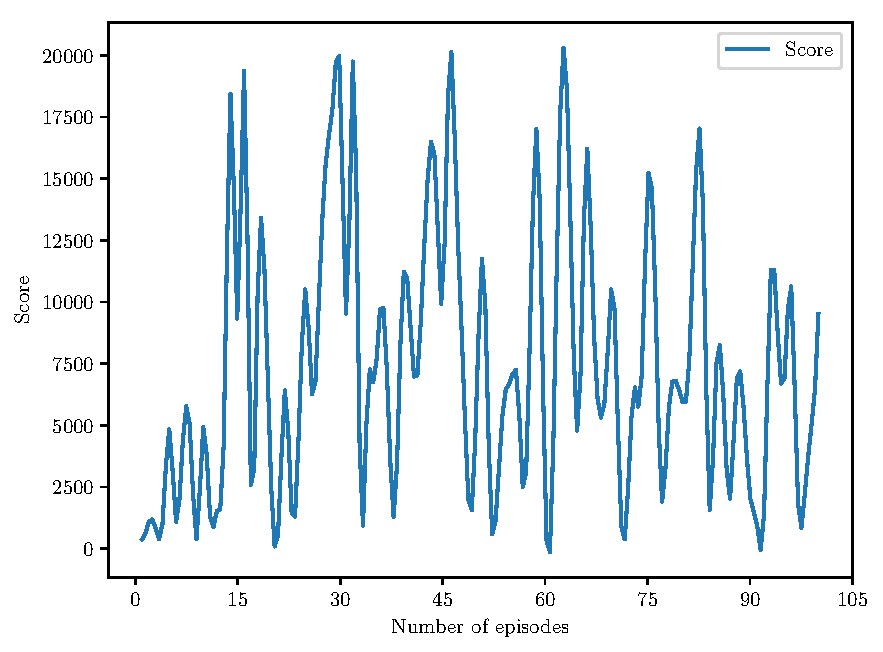
\includegraphics[width=\columnwidth]{plots/subsumption_random.pdf}
		\caption
		{Score achieved by the \textsc{Subsumption} agent with \textsc{Random} exploration.}
		\label{fig:subsumption_random}
	\end{figure}
	
	One problem that was clear with $\epsilon$-greedy exploration is that it can be very slow to learn and waste a great deal of training time in the same states. For example, with $\epsilon$-greedy, Qbert would often oscillate between two adjacent blocks, not seeing the need to explore further until the it randomly chose (with probability $\epsilon$) to explore further. This can be seen in \cref{fig:random_oscillations}, where Qbert is oscillating between the bottom right block and the block to the top right of it. This can explain the slow learning seen in \cref{fig:subsumption_random}.

	\begin{figure}[!htb]
		\centering
		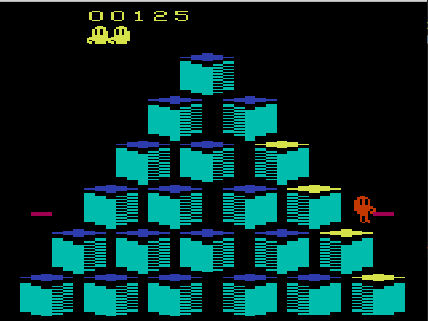
\includegraphics[width=\columnwidth]{screenshots/random_oscillations_2.png}
		\caption
		{Screen capture during Qbert's oscillation between two states.}
		\label{fig:random_oscillations}
	\end{figure}

	The results of the \textsc{Subsumption} agent using \textsc{Optimistic} exploration can be seen in \cref{fig:subsumption_optimistic}. These results are not as encouraging, with the score oscillating around a relatively low value. This can most likely be explained by the fact that we used a relatively simplistic exploration function. With a more sophisticated one, we can most likely obtain better results.
	
	\begin{figure}[!htb]
		\centering
		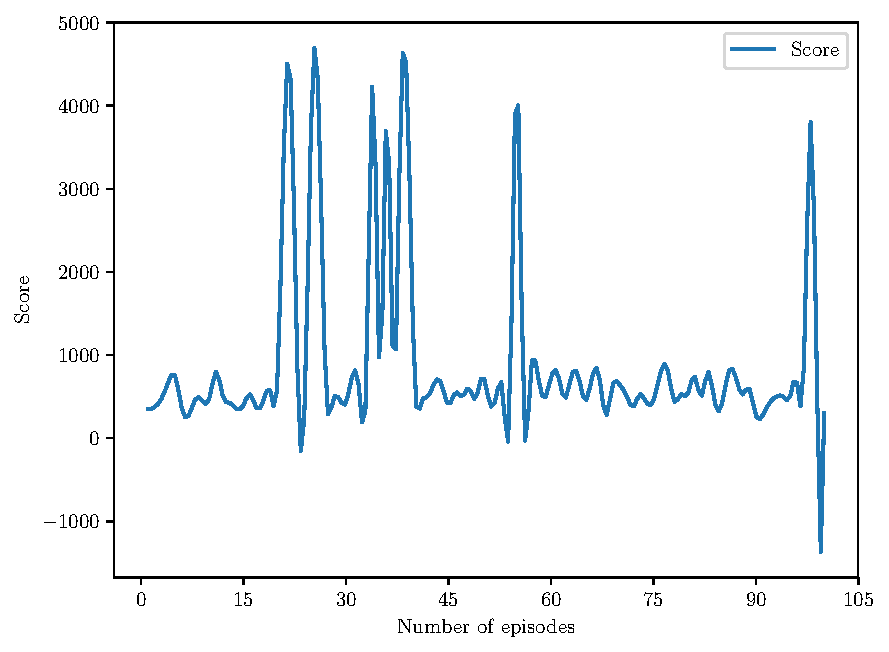
\includegraphics[width=\columnwidth]{plots/subsumption_optimistic.pdf}
		\caption
		{Score achieved by the \textsc{Subsumption} agent with \textsc{Optimistic} exploration.}
		\label{fig:subsumption_optimistic}
	\end{figure}
	
	The results of the \textsc{Subsumption} agent using \textsc{Combined} exploration can be seen in \cref{fig:subsumption_combined}. These results are much more encouraging. We can see the same initial high score values as for \textsc{Random} exploration, with a clear increasing trend. This approach encourages Qbert to visit unexplored states, while also randomly visiting states that may lead to more unexplored states.
	
	\begin{figure}[!htb]
		\centering
		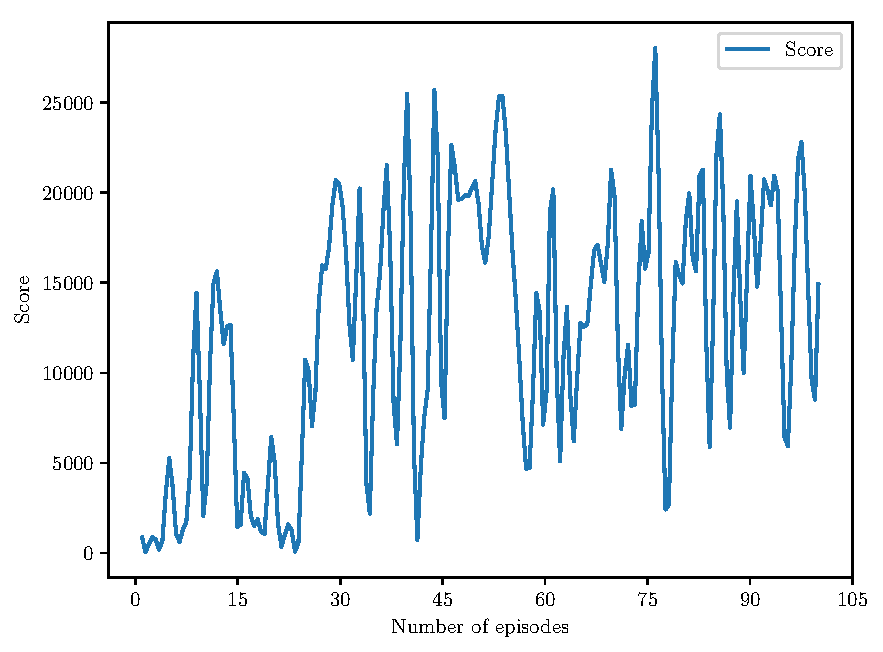
\includegraphics[width=\columnwidth]{plots/subsumption_combined.pdf}
		\caption
		{Score achieved by the \textsc{Subsumption} agent with \textsc{Combined} exploration ($\epsilon$-greedy and optimistic-prior exploration).}
		\label{fig:subsumption_combined}
	\end{figure}
	
	Of course, as described previously, the task of avoiding enemies is itself a good way of exploring the state space and completing a level, since it will force Qbert to jump around the pyramid and visit blocks to make them the right color.
	
	\section{Agent Performance} \label{sec:performance}
	% 30. as above, including analysis of effects of game events on agent behaviour and strategies (e.g., enemy avoidance) AND explanation of results over trials with multiple seeds to demonstrate generalization of learning
	
	Based on the results from the previous sections, it is clear that the \textsc{Subsumption} approach described by Mahadevan and Connell \cite{mahadevan} gives the best results. The model for this approach will now be described in detail.
	
	The agent is separated into three learners: \textsc{EnemyAvoider}, \textsc{FriendlyCatcher} and \textsc{BlockFinder}. The structure is shown in \cref{fig:subsumption}, where the ``S'' suppressor nodes denote priority, i.e., avoiding enemies takes priority over catching friendlies and going on blocks. This approach allows the agent to learn various aspects of the Qbert game independently, with a reduced state space for each task. This separation also makes intuitive sense, since learning how to avoid enemies should have little to do with finding blocks. Combined with the \textsc{Simple} state representation described in \cref{sec:generalization_description}, the \textsc{Subsumption} model can lead to a very small state space which can be learned very quickly.
	
	\begin{figure}[!htb]
		\centering
		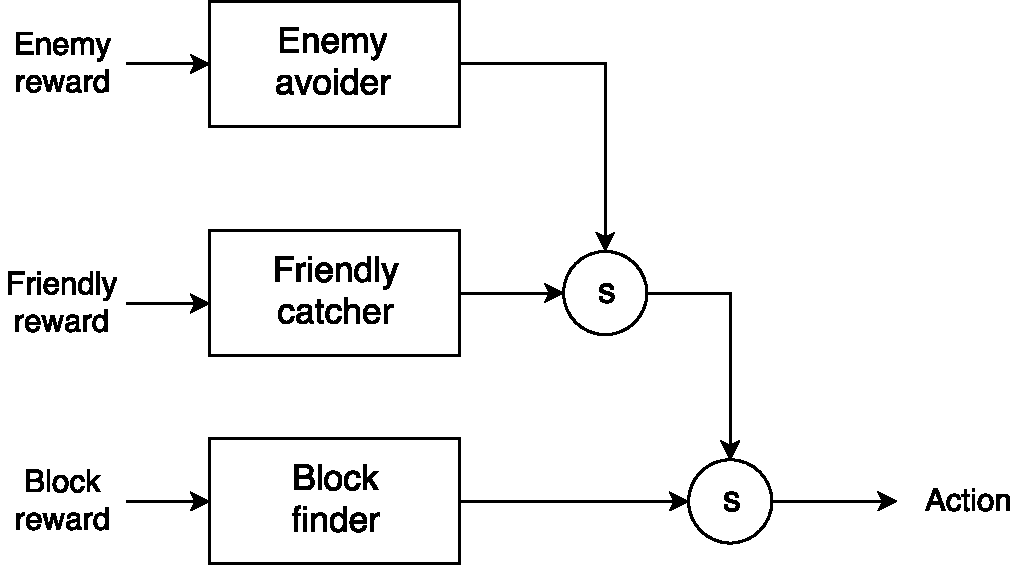
\includegraphics[width=\columnwidth]{plots/subsumption.pdf}
		\caption
		{Subsumption network used by the \textsc{Subsumption} agent.}
		\label{fig:subsumption}
	\end{figure}

	The \textsc{EnemyAvoider} is active whenever an enemy (\textsc{Coily} and \textsc{PurpleBall}) is close to Qbert, i.e. in any of the blocks directly adjacent to Qbert or 2 blocks away. An important strategy is to kill the purple snake enemy (\textsc{Coily}) by jumping on to the floating disks on the left and right of the board. If \textsc{Coily} is nearby, he will jump off the board, giving Qbert 500 points. This maneuver can be seen in \cref{fig:kill_coily}. This score is fed as a reward to the enemy avoider learner. As a penalty for dying to \textsc{Coily}, a negative reward of $-100$ is given to the learner. This combination of positive and negative reinforcement allows the agent to learn how to avoid and kill \textsc{Coily}.
	
	\begin{figure}[!htb]
		\centering
		\includegraphics[width=\columnwidth]{screenshots/kill_coily.png}
		\caption
		{Screen capture during Qbert's jump on a disk to kill Coily.}
		\label{fig:kill_coily}
	\end{figure}

	Indeed, avoiding \textsc{Coily} is probably the most important task to learn in the game. Not only does it prevent Qbert from dying, but it inadvertently makes him explore the entire map while avoiding \textsc{Coily}. This avoidance is essential, and after many runs, the \textsc{Subsumption} agent learns to go back and forth between tiles to out-maneuver \textsc{Coily}. This can be seen in \cref{fig:avoid_coily}.
	
	\begin{figure}[!htb]
		\centering
		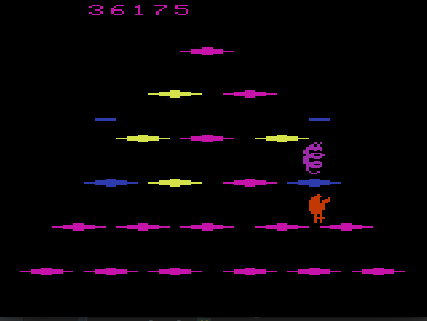
\includegraphics[width=\columnwidth]{screenshots/avoid_coily.png}
		\caption
		{Screen capture during Qbert's back-and-forth maneuver on the bottom corner to avoid \textsc{Coily}.}
		\label{fig:avoid_coily}
	\end{figure}
	
	The \textsc{FriendlyCatcher} is active whenever a friendly green agent (\textsc{Sam} and \textsc{GreenBall}) is within 2 blocks of Qbert. This learner encourages Qbert to catch \textsc{Sam} for 300 points and \textsc{GreenBall} for 100 points. Stopping Sam is also important because he changes the colors of blocks back to their original values, making Qbert do more work.
	
	The \textsc{BlockFinder} is always active and keeps track of the colors of blocks within 2 blocks' distance of Qbert. It specifically keeps track of the number of adjacent blocks that are not of the desired color, encouraging Qbert to change them to their correct color to eventually complete the level. It receives a 25 point reward for turning a block to the goal color, and a 3100 point reward for completing a level.
	
	Note that, although one learner's decision always has priority for executing an action, multiple learners can still learn simultaneously. For example, while Qbert is avoiding an enemy, the block finder learner can still be learning from the actions being taken.
	
	The score results of the \textsc{Subsumption} agent with seeds of 123, 459 and 598 can be seen in \cref{fig:seed123,fig:seed459,fig:seed598}. We can see that the agent performs relatively well for all of these seed values, showing that the agent generalizes well. To fully appreciate the upward trend of learning, it would require more than 100 episodes, but the training is relatively time consuming.
	
	\begin{figure}[!htb]
		\centering
		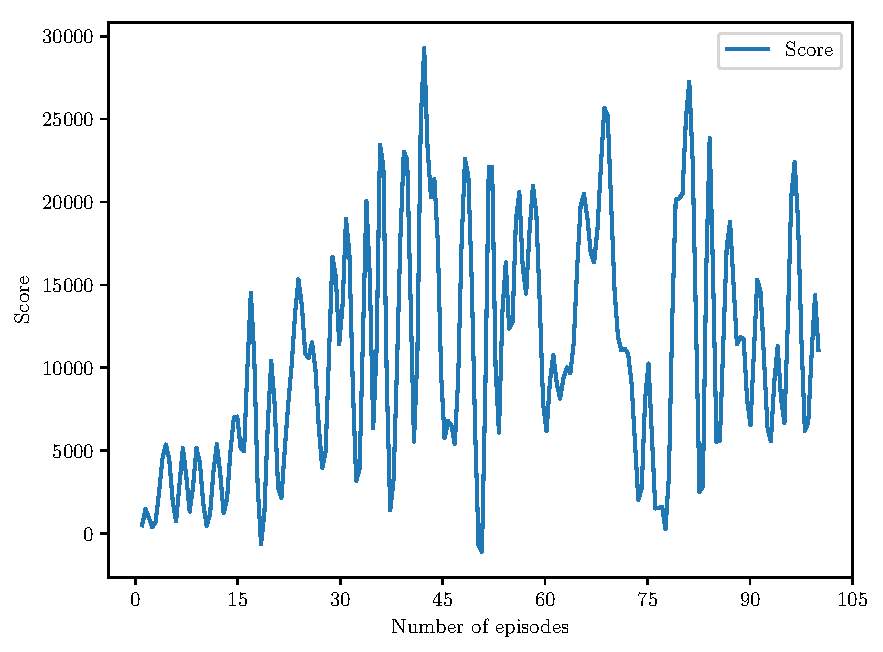
\includegraphics[width=\columnwidth]{plots/seed123.pdf}
		\caption
		{Score achieved by the \textsc{Subsumption} agent with a seed of 123.}
		\label{fig:seed123}
	\end{figure}
	
	\begin{figure}[!htb]
		\centering
		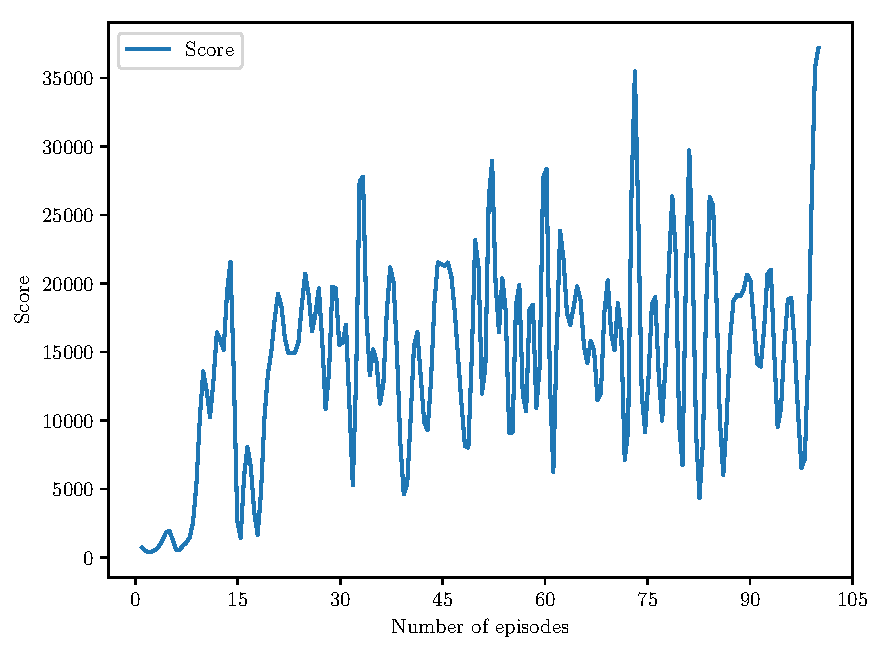
\includegraphics[width=\columnwidth]{plots/seed459.pdf}
		\caption
		{Score achieved by the \textsc{Subsumption} agent with a seed of 459.}
		\label{fig:seed459}
	\end{figure}

	\begin{figure}[!htb]
		\centering
		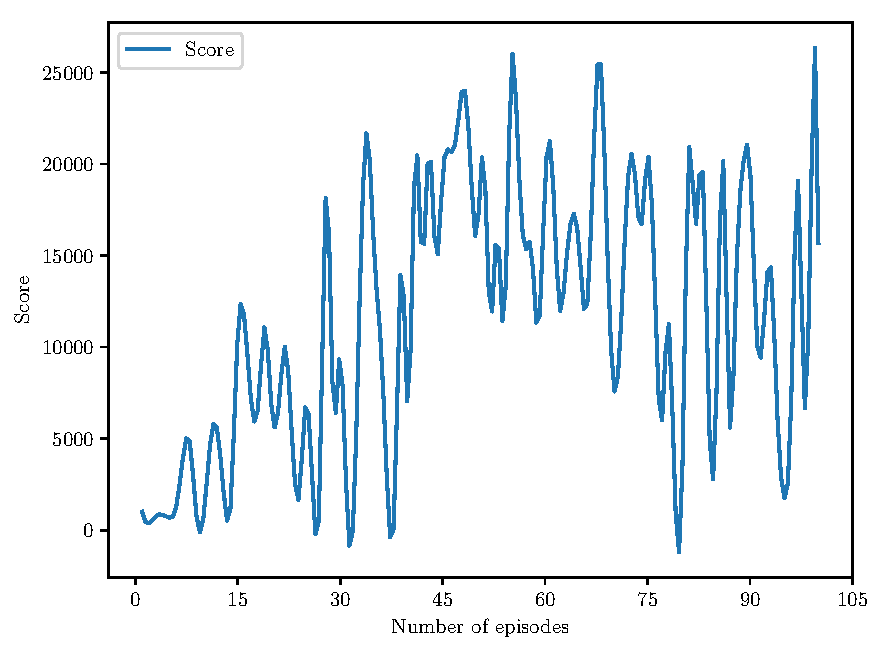
\includegraphics[width=\columnwidth]{plots/seed598.pdf}
		\caption
		{Score achieved by the \textsc{Subsumption} agent with a seed of 598.}
		\label{fig:seed598}
	\end{figure}

	With repeated training, the highest score achieved by the agent is around 41800 and the maximum level reached is 9. There are multiple possible improvements to be made to the agent's behaviour. One would be to discourage it from staying near the top of the pyramid, since this is where \textsc{PurpleBall} spawns. This could possibly be achieved by keeping the \textsc{EnemyAvoider} learner active even when there are no enemies, or only when Qbert is near the top of the pyramid. Another problem is that Qbert doesn't seem to explore very well when he is not avoiding \textsc{Coily}. This could possibly be addressed by encouraging Qbert further to find uncolored blocks by specifying how many blocks are left without the goal color.

	\section*{Acknowledgments}
	There was a discussion with Andrei Purcarus, Andrew Lowther and Juliette Valenchon concerning extracting relevant data from the ALE and high-level learning strategies. Notably, the positions of various important bytes in the ALE RAM were discussed, such as the bytes indicating a safe move update and the byte indicating a level change.
	
	
%	\renewcommand\refname{}
	\bibliographystyle{unsrt}
	\bibliography{readings}{}
	
\end{document}
